\chapter{Implementacja}
\section{Zarządzanie projektem PDDL}
\subsection{Tworzenie projektu PDDL}
\subsection{Tworzenie nowych plików PDDL}
\section{Przetwarzanie kodu PDDL}
\subsection{Wykrywanie błędów składniowych}
\subsection{Tworzenie indeksu}
\subsection{Wykrywanie błędów semantycznych}
\subsection{Podpowiadanie kodu}
\section{Edytor}
\subsection{Kolorowanie kodu}
\subsection{Automatyczne wcięcia}
\subsection{Dopasowanie nawiasów}
\section{Współpraca z oprogramowaniem wyznaczającym plan}
\label{chap:wspolpraca}
Zadaniem oprogramowania wyznaczającego plan (tzw. plannera) jest przetwarzanie problemów automatycznego planowania, uzyskując na wyjściu plan, czyli sekwencję akcji, umożliwiającą osiągnięcie stanu końcowego ze stanu początkowego problemu. Opis problemu wyrażony jest za pomocą języka automatycznego planowania (np. \textit{STRIPS}, \textit{PDDL}). W przypadku języka \textit{PDDL}, wykorzystywanego w niniejszej pracy, zadanie automatycznego planowania składa się z dwóch plików: pliku domeny, w którym opisana jest dziedzina zadania oraz pliku problemu, opisującego stan początkowy oraz docelowy. Współpraca narzędzia GUI4PDDL z plannerami wymaga więc sposobności uzyskania planu na podstawie aktualnej zawartości dwóch, wyżej wymienionych plików. Ponadto należy zagwarantować możliwość zmiany algorytmu planowania lub innych opcji, które są dostępne dla poszczególnych narzędzi. Gotowy plan powinien być również przedstawiony użytkownikowi w postaci czytelnej.

Obecnie dostępnych jest wiele plannerów, korzystających z języka \textit{PDDL}, różniących się dostępnymi algorytmami, sposobem uruchamiania, ilością oraz rodzajem przyjmowanych na wejściu argumentów, a także strukturą strumienia wyjściowego. Ze względu na to, że programy wyznaczające plan tworzone są często z przeznaczeniem na konkurs \textit{IPC} (\textit{International Planning Competition} \textbf{ODNOŚNIK DO PUNKTU O IPC}), dotychczas nie zdefiniowano standardu uruchamiania tego typu narzędzi, który obejmowałby m.in. ujednolicenie argumentów linii poleceń, wykorzystywanych, dodatkowych narzędzi, specyficznych dla systemu operacyjnego oraz formatu plików wyjściowych.

Analiza przykładowych narzędzi (\textit{FastDownward}, \textit{SATPLAN}, \textit{FastForward})(\textbf{MOŻE ZNALEŹĆ WIĘCEJ PLANNERÓW I SPRAWDZIĆ?}) pod kątem inicjalizacji procesu planowania wykazała następujące cechy wspólne oraz różnice pomiędzy plannerami:
\begin{table}[h]
\centering
\caption{Cechy wspólne oraz różnice w uruchamianiu pomiędzy przykładowymi plannerami.}
\label{plannersTable}
\begin{tabular}{|p{6cm}|p{6cm}|}
\hline
\multicolumn{1}{|>{\centering\arraybackslash}m{6cm}|}{\textbf{Cechy wspólne}} 
    & \multicolumn{1}{>{\centering\arraybackslash}m{6cm}|}{\textbf{Różnice}} 
   \\
   \hline
\begin{itemize}
\item Narzędzia konsolowe.
\item Wymaganie wskazania ścieżek do plików domeny oraz problemu.
\item Możliwość wyboru algorytmu za pomocą argumentu wejściowego programu.
\item Tworzenie pliku wyjściowego z wynikowym planem.
\end{itemize}
&
\begin{itemize}
\item Różna liczba faz przetwarzania.
\item Różna liczba podprogramów plannera.
\item Różnice w nazewnictwie poszczególnych opcji i algorytmów.
\item Różnice w nazwie pliku wyjściowego oraz jego formatowaniu.
\end{itemize} \\
\hline
\end{tabular}
\end{table}

Biorąc pod uwagę powyższe cechy wspólne oraz wymaganie projektu, dotyczące możliwości integracji z wieloma plannerami, ze szczególnym uwzględnieniem \textit{FastDownward}, zdecydowano o stworzeniu wewnętrznego standardu uruchamiania. Standard ten opisuje postać argumentów linii poleceń dla plików plannerów, które mogą być prawidłowo powiązane z wtyczką GUI4PDDL. 

Narzędzia te wymagają podania na wejście programu ścieżek do plików domeny oraz problemu. W niektórych przypadkach konieczne jest także wskazanie nazwy algorytmu planowania. Cechy te w całości pokrywają się z wymaganiami skryptu uruchomieniowego narzędzia \textit{FastDownward}. W związku z tym, powzięto decyzję o przyjęciu formatu skryptu uruchomieniowego, analogicznego do formatu skryptu \texttt{plan}, znajdującego się w katalogu \texttt{src} \textit{FastDownward}. Skrypt (bądź bezpośrednio plik wykonywalny plannera) przeznaczony do integracji z wtyczką GUI4PDDL musi więc przyjmować następujące argumenty wejściowe w odpowiedniej kolejności:

\noindent
\centerline{\texttt{<ścieżka\_do\_domeny>}\textvisiblespace\texttt{<ścieżka\_do\_problemu>}\textvisiblespace\texttt{<argumenty\_planowania>}}


\noindent
gdzie:
\begin{itemize}
\item \textbf{\texttt{<ścieżka\_do\_domeny>}} -- ścieżka do pliku domeny danego zadania automatycznego planowania.
\item \textbf{\texttt{<ścieżka\_do\_problemu>}} -- ścieżka do pliku problemu, zdefiniowanego na dziedzinie wskazanej w podanym jako pierwszy argument pliku domeny.
\item \textbf{\texttt{<argumenty\_planowania>}} -- dowolne argumenty plannera, na przykład dotyczące wyboru algorytmu planowania.
\end{itemize}
Narzędzia uruchamiane według innego schematu nie będą prawidłowo zintegrowane z GUI4PDDL. W takim przypadku należy przygotować skrypt powłoki systemu operacyjnego, który dostosuje sposób inicjalizacji procesu planowania do przedstawionego powyżej. Dzięki zastosowaniu funkcji systemowych (roz.~\ref{chap:przerywanie}) istnieje możliwość kontroli nad tego typu skryptami z poziomu Eclipse, włączając uruchamiane przez nie podprocesy. 

Poza określonym formatem argumentów linii poleceń, każdy planner musi zapewnić możliwość zapisu uzyskanego planu do pliku w postaci czytelnej, co jest wykorzystywane w przeglądarce planów, opisanej w rozdziale~\ref{chap:zew_oprogr}.

\subsection{Konfiguracja zewnętrznego oprogramowania}

Istnienie zróżnicowanego oprogramowania, pozwalającego wyznaczyć plan wymaga możliwości integracji ze środowiskiem programistycznym. Platforma Eclipse zapewnia standardową opcję uruchamiania zewnętrznych narzędzi z poziomu menu ,,Run'' aplikacji, bądź skrótów znajdujących się na pasku narzędziowym lub menu kontekstowym edytowanego pliku. W wielu wtyczkach, rozszerzających Eclipse o obsługę języków programowania ogólnego przeznaczenia (Java, C++), opcja ta odpowiada za rozpoczęcie procesu kompilacji. Biorąc pod uwagę podobieństwo procesu planowania do kompilacji oraz przyzwyczajenia użytkowników, zdecydowano o wprowadzeniu w projekcie GUI4PDDL analogicznego sposobu uruchamiania plannera i jego konfiguracji.

Zanim możliwa będzie aktywacja planowania z poziomu Eclipse, należy skonfigurować planner, wybierając z menu ,,Window'', opcję ,,Preferences'', a następnie w otwartym oknie, rozwijając listę ,,PDDL'' wybrać element ,,Planners''.

\newpage
\begin{figure}[h!]
    \centering
    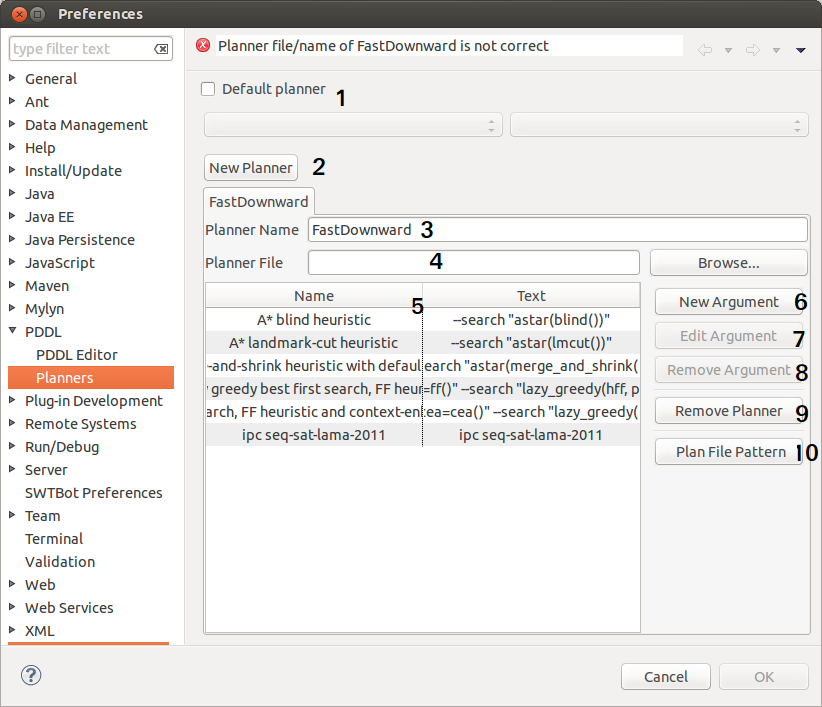
\includegraphics[width=\textwidth]{img/planner_preferences_window}
    \caption{Widok okna konfiguracji plannera.}
    \label{fig:preferences_window}
\end{figure}
Standardowo, dostępny jest wstępnie skonfigurowany planner \textit{FastDownward}. Okno preferencji udostępnia następujące opcje:
\begin{enumerate}
\item Wybór plannera domyślnego. Włączenie tej opcji, powoduje, że przy każdym uruchomieniu procesu planowania na plikach domeny i problemu, wykorzystany będzie wskazany w tym polu planner wraz z odpowiednim algorytmem planowania.
\item Nowa konfiguracja. Przycisk ten umożliwia stworzenie nowej konfiguracji, dla innego niż bieżący plannera. Może istnieć wiele takich konfiguracji, które w trakcie uruchamiania planowania można dowolnie zmieniać.
\item Nazwa konfiguracji. Pozwala na rozróżnienie poszczególnych konfiguracji. Nazwa powinna być unikalna i może składać się z liter, cyfr, spacji oraz znaków ,,.'', ,,\_'', ,,-''.
\item Ścieżka do pliku plannera. Za pomocą przycisku ,,Browse...'' należy wskazać ścieżkę do pliku wykonywalnego lub skryptu powłoki systemu operacyjnego (Linux lub Windows), zgodnego z formatem przedstawionym w rozdziale~\ref{chap:wspolpraca}.
\item Argumenty plannera. W pierwszej kolumnie znajduje się czytelna dla użytkownika nazwa argumentu, w szczególności nazwa wykorzystywanego algorytmu planowania, która będzie używana jako prosty odpowiednik argumentu linii poleceń, znajdującego się w drugiej kolumnie. Parametry wiersza poleceń danego plannera wpisane muszą być w sposób identyczny, jak przy wpisywaniu ich podczas uruchamiania w konsoli.
\item Nowy argument. Przycisk ten umożliwia dodanie nowego argumentu linii poleceń plannera wraz z jego nazwą.
\item Edycja argumentu. Pozwala na edycję aktualnie zaznaczonego argumentu plannera.
\item Usunięcie argumentu. Pozwala na usunięcie aktualnie zaznaczonego argumentu plannera.
\item Usunięcie konfiguracji plannera. Przycisk ten usuwa bieżącą konfigurację. Nie ma możliwości cofnięcia tej operacji, dlatego przed jej wykonaniem wyświetlone zostaje pytanie, potwierdzające chęć usunięcia konfiguracji.
\item Wzorzec pliku planu. Okno to umożliwia zdefiniowanie wyrażenia regularnego, dotyczącego nazwy pliku wynikowego planu, powstałego w rezultacie działania bieżącego plannera. Prawidłowy wzorzec pozwala na wykrycie plików planów i bezpośrednie ich wyświetlenie przy pomocy przeglądarki planów (roz.~\ref{chap:zew_oprogr}).
\begin{figure}[h!]
    \centering
    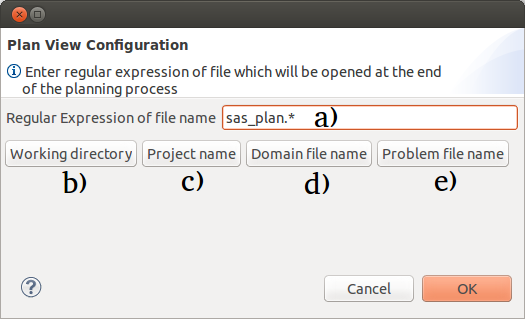
\includegraphics[width=0.8\textwidth]{img/plan_view_dialog}
    \caption{Widok okna konfiguracji przeglądarki planów.}
    \label{fig:plan_view_window}
\end{figure}
\begin{enumerate}
\item Wyrażenie regularne. Wzorzec opisujący nazwę pliku wynikowego planu. Planner \textit{FastDownward} standardowo generuje pliki planów o nazwie ,,sas\_plan.'', a w przypadku większej ilości planów kolejno ,,sas\_plan.1'', ,,sas\_plan.2''..., dlatego wyrażenie obejmujące te nazwy ma postać ,,sas\_plan.*''.
\item Wzorzec katalogu roboczego. Przycisk ten powoduje wstawienie w bieżącym miejscu kursora, ciągu ,,-working\_directory-'', który w czasie procesu planowania zamieniany jest na aktualną nazwę katalogu roboczego plannera (roz.~\ref{chap:zew_oprogr}). Opcja ta pozwala na wykrycie plików wynikowych, które jako swoją nazwę przyjmują nazwę bieżącego katalogu.
\item Wzorzec nazwy projektu. Przycisk ten powoduje wstawienie w bieżącym miejscu kursora, ciągu ,,-project\_name-'', który w czasie planowania zamieniany jest na nazwę projektu Eclipse, w którym znajdują się przetwarzane pliki domeny oraz problemu.
\item Wzorzec nazwy pliku domeny. Przycisk ten powoduje wstawienie w bieżącym miejscu kursora, ciągu ,,-domain\_file\_name-'', który w czasie planowania zamieniany jest na nazwę pliku domeny, wykorzystywanej w tym przetwarzaniu, bez rozszerzenia ,,.pddl''.
\item Wzorzec nazwy pliku problemu. Przycisk ten powoduje wstawienie w bieżącym miejscu kursora, ciągu ,,-problem\_file\_name-'', który w czasie planowania zamieniany jest na nazwę pliku problemu, wykorzystywanego w tym przetwarzaniu, bez rozszerzenia ,,.pddl''.
\end{enumerate}
\end{enumerate}

Minimalna konfiguracja plannera, możliwa do zapisu składa się z prawidłowej nazwy oraz ścieżki do pliku programu. Zachowanie utworzonych lub zmodyfikowanych ustawień odbywa się po naciśnięciu przycisku ,,OK''.
Wszystkie konfiguracje zapisywane są w tzw. obszarze stanu (ang. \textit{state area}) przestrzeni roboczej (ang. \textit{workspace}) w folderze \path{planner_preferences}. 

Ścieżka do tego katalogu ma następującą postać:

\noindent
\centerline{\path{<l_p_rob>/.metadata/.plugins/pl.poznan.put.cs.gui4pddl/planner_preferences}}

\noindent
gdzie:

\noindent
\textbf{\path{<l_p_rob>}} -- lokalizacja przestrzeni roboczej.

Każda konfiguracja ustawień plannera zapisywana jest w osobnym pliku o nazwie analogicznej do wpisanej w oknie preferencji. Ze względu na łatwość modyfikacji, elastyczność w przechowywaniu listy argumentów oraz odporność na zmiany, jako format zapisu danych wybrano XML. Do tego typu serializacji, wykorzystane zostało dołączone do platformy Eclipse API Memento. W tej formie zapisywane są wszystkie informacje o konfiguracji, z wyjątkiem ustawień domyślnego plannera, które zachowywane są przy pomocy standardowego API Eclipse do zapisu preferencji -- \textit{Preferences}.

\lstset{language=XML}          % Set your language (you can change the language for each code-block optionally)
\begin{lstlisting}[frame=single,caption={Przykładowa konfiguracja plannera FastDownward w postaci XML}]  % Start your code-block
<?xml version="1.0" encoding="UTF-8"?>
<PlannerPreferences 
	PlanViewFilePattern="sas_plan.*" 
	PlannerFilePath="/home/user/fast-downward/src/plan" 
	PlannerName="FastDownward">
	<PlannerArguments>
		<PlannerArgumentsEntry 
			PlannerArgumentKey="A* blind heuristic" 
			PlannerArgumentValue="--search &quot;astar(blind())&quot;"/>
		<PlannerArgumentsEntry 
			PlannerArgumentKey="ipc seq-sat-lama-2011" 
			PlannerArgumentValue="ipc seq-sat-lama-2011"/>
	</PlannerArguments>
</PlannerPreferences>
\end{lstlisting}



\subsection{Uruchamianie zewnętrznego oprogramowania}
\label{chap:zew_oprogr}
\subsection{Przerywanie procesu planowania}
\label{chap:przerywanie}
